% Prime k-tuples against the Hardy-Littlewood prediction (generated by a script).
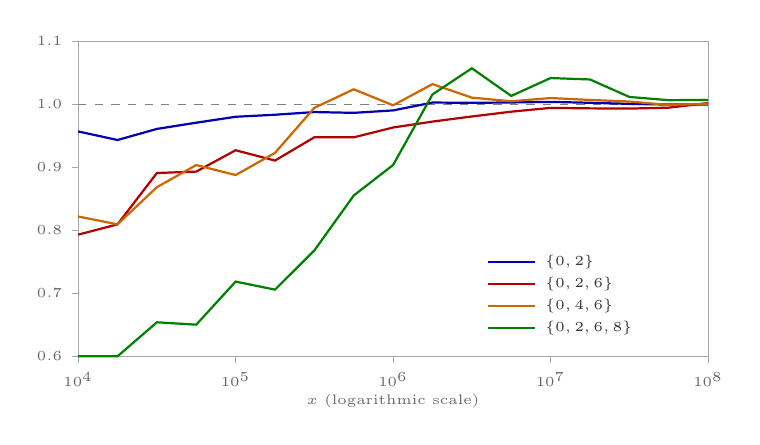
\begin{tikzpicture}[x=1cm,y=1cm]
\draw[black!35] (0,0) rectangle (8.00,4.00);
\draw[black!35] (0,0.00)--(-0.08,0.00) node[left,font=\tiny,black!60]{$0.6$};
\draw[black!35] (0,0.80)--(-0.08,0.80) node[left,font=\tiny,black!60]{$0.7$};
\draw[black!35] (0,1.60)--(-0.08,1.60) node[left,font=\tiny,black!60]{$0.8$};
\draw[black!35] (0,2.40)--(-0.08,2.40) node[left,font=\tiny,black!60]{$0.9$};
\draw[black!35] (0,3.20)--(-0.08,3.20) node[left,font=\tiny,black!60]{$1.0$};
\draw[black!35] (0,4.00)--(-0.08,4.00) node[left,font=\tiny,black!60]{$1.1$};
\draw[black!35] (0.00,0)--(0.00,-0.08) node[below,font=\tiny,black!60]{$10^{4}$};
\draw[black!35] (2.00,0)--(2.00,-0.08) node[below,font=\tiny,black!60]{$10^{5}$};
\draw[black!35] (4.00,0)--(4.00,-0.08) node[below,font=\tiny,black!60]{$10^{6}$};
\draw[black!35] (6.00,0)--(6.00,-0.08) node[below,font=\tiny,black!60]{$10^{7}$};
\draw[black!35] (8.00,0)--(8.00,-0.08) node[below,font=\tiny,black!60]{$10^{8}$};
\node[below,font=\tiny,black!60] at (4.00,-0.35) {$x$ (logarithmic scale)};
\draw[black!50,dashed] (0,3.20)--(8.00,3.20);
\draw[blue!70!black,thick] (0.000,2.856) -- (0.500,2.747) -- (1.000,2.888) -- (1.500,2.967) -- (2.000,3.042) -- (2.500,3.068) -- (3.000,3.102) -- (3.500,3.092) -- (4.000,3.123) -- (4.500,3.223) -- (5.000,3.219) -- (5.500,3.224) -- (6.000,3.231) -- (6.500,3.220) -- (7.000,3.206) -- (7.500,3.197) -- (8.000,3.199);
\draw[blue!70!black,thick] (5.20,1.20)--(5.80,1.20) node[right,font=\tiny,black!80]{$\{0,2\}$};
\draw[red!70!black,thick] (0.000,1.545) -- (0.500,1.676) -- (1.000,2.328) -- (1.500,2.346) -- (2.000,2.617) -- (2.500,2.486) -- (3.000,2.782) -- (3.500,2.781) -- (4.000,2.906) -- (4.500,2.981) -- (5.000,3.046) -- (5.500,3.107) -- (6.000,3.155) -- (6.500,3.149) -- (7.000,3.146) -- (7.500,3.158) -- (8.000,3.216);
\draw[red!70!black,thick] (5.20,0.92)--(5.80,0.92) node[right,font=\tiny,black!80]{$\{0,2,6\}$};
\draw[orange!80!black,thick] (0.000,1.776) -- (0.500,1.676) -- (1.000,2.148) -- (1.500,2.429) -- (2.000,2.302) -- (2.500,2.583) -- (3.000,3.156) -- (3.500,3.391) -- (4.000,3.188) -- (4.500,3.457) -- (5.000,3.285) -- (5.500,3.239) -- (6.000,3.280) -- (6.500,3.256) -- (7.000,3.236) -- (7.500,3.192) -- (8.000,3.209);
\draw[orange!80!black,thick] (5.20,0.64)--(5.80,0.64) node[right,font=\tiny,black!80]{$\{0,4,6\}$};
\draw[green!50!black,thick] (0.000,0.000) -- (0.500,0.000) -- (1.000,0.432) -- (1.500,0.402) -- (2.000,0.949) -- (2.500,0.847) -- (3.000,1.345) -- (3.500,2.042) -- (4.000,2.430) -- (4.500,3.326) -- (5.000,3.658) -- (5.500,3.307) -- (6.000,3.534) -- (6.500,3.516) -- (7.000,3.294) -- (7.500,3.253) -- (8.000,3.256);
\draw[green!50!black,thick] (5.20,0.36)--(5.80,0.36) node[right,font=\tiny,black!80]{$\{0,2,6,8\}$};
\end{tikzpicture}
